\documentclass[border=6pt]{standalone}
\usepackage{amsmath}
\usepackage{tikz}
\usetikzlibrary{arrows.meta}
\begin{document}
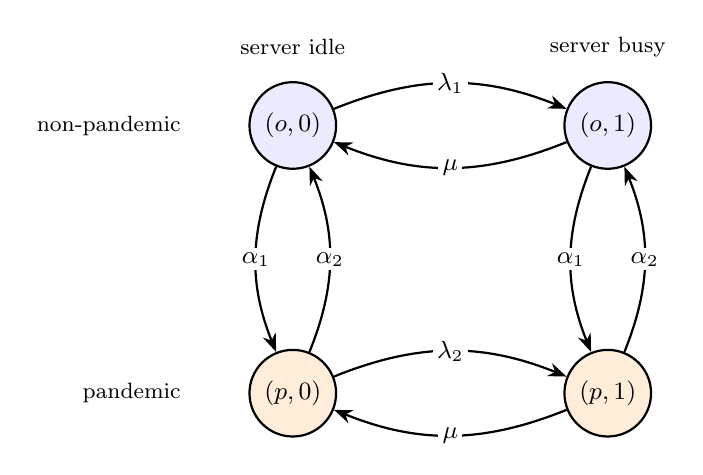
\begin{tikzpicture}[>=Stealth,font=\small,
 s/.style={draw,thick,circle,minimum size=1.1cm,inner sep=0pt,fill=blue!8},
 e/.style={->,thick},
 lab/.style={font=\small,fill=white,inner sep=1.5pt},
 every loop/.style={->,thick,looseness=6}]
\node[s] (o0) at (0,0) {$(o,0)$};
\node[s] (o1) at (4,0) {$(o,1)$};
\node[s,fill=orange!15] (p0) at (0,-3.4) {$(p,0)$};
\node[s,fill=orange!15] (p1) at (4,-3.4) {$(p,1)$};
\draw[e] (o0) to[bend left=22] node[lab]{$\lambda_1$} (o1);
\draw[e] (o1) to[bend left=22] node[lab]{$\mu$} (o0);
\draw[e] (p0) to[bend left=22] node[lab]{$\lambda_2$} (p1);
\draw[e] (p1) to[bend left=22] node[lab]{$\mu$} (p0);
\draw[e] (o0) to[bend right=22] node[lab]{$\alpha_1$} (p0);
\draw[e] (p0) to[bend right=22] node[lab]{$\alpha_2$} (o0);
\draw[e] (o1) to[bend right=22] node[lab]{$\alpha_1$} (p1);
\draw[e] (p1) to[bend right=22] node[lab]{$\alpha_2$} (o1);
\node[font=\footnotesize,anchor=east] at (-1.3,0) {non-pandemic};
\node[font=\footnotesize,anchor=east] at (-1.3,-3.4) {pandemic};
\node[font=\footnotesize] at (0,1.0) {server idle};
\node[font=\footnotesize] at (4,1.0) {server busy};
\end{tikzpicture}
\end{document}
